% This is "sig-alternate.tex" V2.0 May 2012
% This file should be compiled with V2.5 of "sig-alternate.cls" May 2012
%
% This example file demonstrates the use of the 'sig-alternate.cls'
% V2.5 LaTeX2e document class file. It is for those submitting
% articles to ACM Conference Proceedings WHO DO NOT WISH TO
% STRICTLY ADHERE TO THE SIGS (PUBS-BOARD-ENDORSED) STYLE.
% The 'sig-alternate.cls' file will produce a similar-looking,
% albeit, 'tighter' paper resulting in, invariably, fewer pages.
%
% ----------------------------------------------------------------------------------------------------------------
% This .tex file (and associated .cls V2.5) produces:
%       1) The Permission Statement
%       2) The Conference (location) Info information
%       3) The Copyright Line with ACM data
%       4) NO page numbers
%
% as against the acm_proc_article-sp.cls file which
% DOES NOT produce 1) thru' 3) above.
%
% Using 'sig-alternate.cls' you have control, however, from within
% the source .tex file, over both the CopyrightYear
% (defaulted to 200X) and the ACM Copyright Data
% (defaulted to X-XXXXX-XX-X/XX/XX).
% e.g.
% \CopyrightYear{2007} will cause 2007 to appear in the copyright line.
% \crdata{0-12345-67-8/90/12} will cause 0-12345-67-8/90/12 to appear in the copyright line.
%
% ---------------------------------------------------------------------------------------------------------------
% This .tex source is an example which *does* use
% the .bib file (from which the .bbl file % is produced).
% REMEMBER HOWEVER: After having produced the .bbl file,
% and prior to final submission, you *NEED* to 'insert'
% your .bbl file into your source .tex file so as to provide
% ONE 'self-contained' source file.
%
% ================= IF YOU HAVE QUESTIONS =======================
% Questions regarding the SIGS styles, SIGS policies and
% procedures, Conferences etc. should be sent to
% Adrienne Griscti (griscti@acm.org)
%
% Technical questions _only_ to
% Gerald Murray (murray@hq.acm.org)
% ===============================================================
%
% For tracking purposes - this is V2.0 - May 2012

\documentclass{sig-alternate}
\usepackage{nameref}
\usepackage[usenames]{color}

\newcommand{\basicalert}[2]{\fbox{\bfseries\sffamily\scriptsize\color{blue} #1}{\sf\small$\blacktriangleright$\textit{\color{red} #2}$\blacktriangleleft$} }
\newcommand{\mika}[1]{\basicalert{From Mika}{#1}}
\newcommand{\eetu}[1]{\basicalert{From Eetu}{#1}}
%\newcommand{\mika}[1]{\ignorespaces}
%\newcommand{\eetu}[1]{\ignorespaces}

\begin{document}
%
% --- Author Metadata here ---
\conferenceinfo{WOODSTOCK}{'97 El Paso, Texas USA}
%\CopyrightYear{2007} % Allows default copyright year (20XX) to be over-ridden - IF NEED BE.
%\crdata{0-12345-67-8/90/01}  % Allows default copyright data (0-89791-88-6/97/05) to be over-ridden - IF NEED BE.
% --- End of Author Metadata ---


\title{Agile metrics: How and why}
%\subtitle{[Extended Abstract]
%\titlenote{A full version of this paper is available as
%\textit{Author's Guide to Preparing ACM SIG Proceedings Using
%\LaTeX$2_\epsilon$\ and BibTeX} at
%\texttt{www.acm.org/eaddress.htm}}}

%
% You need the command \numberofauthors to handle the 'placement
% and alignment' of the authors beneath the title.
%
% For aesthetic reasons, we recommend 'three authors at a time'
% i.e. three 'name/affiliation blocks' be placed beneath the title.
%
% NOTE: You are NOT restricted in how many 'rows' of
% "name/affiliations" may appear. We just ask that you restrict
% the number of 'columns' to three.
%
% Because of the available 'opening page real-estate'
% we ask you to refrain from putting more than six authors
% (two rows with three columns) beneath the article title.
% More than six makes the first-page appear very cluttered indeed.
%
% Use the \alignauthor commands to handle the names
% and affiliations for an 'aesthetic maximum' of six authors.
% Add names, affiliations, addresses for
% the seventh etc. author(s) as the argument for the
% \additionalauthors command.
% These 'additional authors' will be output/set for you
% without further effort on your part as the last section in
% the body of your article BEFORE References or any Appendices.

\numberofauthors{3} %  in this sample file, there are a *total*
% of EIGHT authors. SIX appear on the 'first-page' (for formatting
% reasons) and the remaining two appear in the \additionalauthors section.
%
\author{
% You can go ahead and credit any number of authors here,
% e.g. one 'row of three' or two rows (consisting of one row of three
% and a second row of one, two or three).
%
% The command \alignauthor (no curly braces needed) should
% precede each author name, affiliation/snail-mail address and
% e-mail address. Additionally, tag each line of
% affiliation/address with \affaddr, and tag the
% e-mail address with \email.
%
% 1st. author
\alignauthor
Eetu Kupiainen\\
       \affaddr{Aalto University}\\
       \affaddr{Konemiehentie 2}\\
       \affaddr{Espoo, Finland}\\
       \email{eetu.kupiainen@aalto.fi}
% 2nd. author
\alignauthor
Mika M�ntyl�\\
       \affaddr{Aalto University}\\
       \affaddr{Konemiehentie 2}\\
       \affaddr{Espoo, Finland}\\
       \email{mika.mantyla@aalto.fi}
% 3rd. author
\alignauthor Juha Itkonen\\
       \affaddr{Aalto University}\\
       \affaddr{Konemiehentie 2}\\
       \affaddr{Espoo, Finland}\\
       \email{juha.itkonen@aalto.fi}
}
% There's nothing stopping you putting the seventh, eighth, etc.
% author on the opening page (as the 'third row') but we ask,
% for aesthetic reasons that you place these 'additional authors'
% in the \additional authors block, viz.
%\additionalauthors{Additional authors: John Smith (The Th{\o}rv{\"a}ld Group,
%email: {\texttt{jsmith@affiliation.org}}) and Julius P.~Kumquat
%(The Kumquat Consortium, email: {\texttt{jpkumquat@consortium.net}}).}
%\date{30 July 1999}
% Just remember to make sure that the TOTAL number of authors
% is the number that will appear on the first page PLUS the
% number that will appear in the \additionalauthors section.

\maketitle
\begin{abstract}

\end{abstract}

% A category with the (minimum) three required fields
\category{H.4}{Information Systems Applications}{Miscellaneous}
%A category including the fourth, optional field follows...
\category{D.2.8}{Software Engineering}{Metrics}[agile metrics]

\terms{Theory}

\keywords{ACM proceedings, \LaTeX, text tagging}

\section{Introduction}

% Software engineering is at a crossroads as there are new leaner and more
% agile software development methods appearing next to the traditional
% software development methods.
\mika{Kappaleen pointti: No literature reviews of actual metric use}
Software metrics have been studied for decades and several literature reviews
have been published.
Yet, the literature reviews have been written from an academic viewpoint that
typically focuses on the effectiveness of a single metric. For example, Catal
et al review fault prediction metrics \cite{catal2009systematic}, Purao et al
review metrics for object oriented systems\cite{purao2003product} and
Kitchenham performs a mapping of most cited software metrics
papers\cite{kitchenham_whats_2010}. To our knowledge there are no systematic
literature reviews on the actual use of software metrics in the industry.

\mika{Kappaleen pointti: Agile on t�rke�� eik� metriikkoja tutkittu}
Agile software development is becoming increasing popular in the software
industry. The agile approach seems to be contradicting with the traditional
metrics approaches. However, at the same time agile software development
highlights some measures that should be used, e.g. burndown graphs and 100\%
automated unit testing coverage. However, measurement research with agile
methods remains scarce.

The goal of this paper is to review the literature of actual use of software
metrics in the context of agile software development. This study will lay out
the current state of industrial agile metric papers. Moreover, the study
uncovers the reasons for metrics usage as well as highlights actions that the
use of metrics can trigger. Due to our research goal, we are more interested
in case studies and actual empirical findings than unproven theories or
models.

This paper is structured as follows. Section...

\section{Background}

\subsection{Evidence based software engineering}

\subsection{Measurement}
According to Fenton et al.\cite{fenton1998software} ``Measurement is the
process by which numbers of symbols are assigned to attributes of entities in
the real world in such way as to describe them according to clearly defined
rules.''


\subsection{Previous metric research}

There are a few mapping studies on software metrics(t�h�n vois lis�t� kitch
whats 2010:ss� olevat muut mut en tii� mit� lis�arvoa ne tois).
\cite{kitchenham_whats_2010} says there is a large body of research related to
software metrics. However, she highlights that all evidence should be
critically appraised so that further studies can be based on good quality
evidence. She also reminds researchers to understand the context where metrics
are taken from - failure to understand context will probably not provide
answers to industry-related questions. 



--EBSE
--Mittaamisen SR:t
--Agile mittaamisen muut tutkimukset vai enemm�nkin tutkimuksessa k�ytettyjen
termien ja k�sitteiden selitt�minen
 --Aims and research questions


\subsection{Aims and research questions}
The aim of this paper is to provide preliminary results from a systematic
review (SR) on agile metrics. Moreover, we are interested on the
industrial use of metrics in agile context.

The performed SR has more research questions but for this paper only
the following questions are considered:

\begin{enumerate}
  \item Why are metrics used?
  \item What actions do the use of metrics trigger?
  \item Which metrics are used?
\end{enumerate}

\section{Review method}
SR was chosen as research method because we are trying to understand a problem
instead of trying to find a solution to it. Also, there was already
existing literature that could be synthesized.

\subsection{Protocol development}
Kitchenham's guide for SRs\cite{kitchenham2004procedures} was used as a basis
for developing the review protocol. Additionally, other
guidelines\cite{webster2002analyzing}, a lessons learned from SRs
\cite{brereton2007lessons}, a SR case\cite{dyba_empirical_2008} and a SR
on SR\cite{kitchenham2013systematic} were used to further understand the
challenges and opportunities of SRs. 

The protocol was also iterated in weekly meetings with the researchers, as
well as in a pilot described in \ref{pilot}.

\subsection{Search and selection process}

The strategy for finding primary studies was following:

\begin{enumerate}
  \item Initial check that there are enough papers to conduct SR
  \item Stage 1: Automated search
  \item Pilot
  \item Stage 2: Include and exclude based on title and abstract
  \item Stage 3: Include and exclude based on full text. Conduct data
  extraction and quality assessment.
\end{enumerate}

Table \ref{SelectionFunnel} shows the selection funnel in terms of amount
papers.

%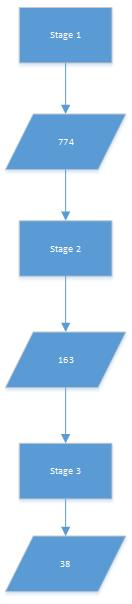
\includegraphics{SelectionFunnel.jpg}

\begin{table}
\centering
\caption{Paper selection funnel}
\begin{tabular}{|l|c|r} \hline
\label{SelectionFunnel}
\textbf{Phase} & \textbf{Amount of papers} \\ \hline
Phase 1 & 774 \\ \hline 
Phase 2 & 163 \\ \hline
Phase 3 & 39\\
\hline
\end{tabular}
\end{table}


\subsubsection{Search strings}
Scopus was used to find the primary documents with automated search. The first
search string was:

TITLE-ABS-KEY(software AND (agile OR lean OR "crystal method" OR "crystal
clear" OR dsdm OR "dynamic systems development method" OR fdd OR "feature
driven development" OR "agile unified process" OR "agile modeling" OR scrumban
OR kanban OR scrum OR "extreme programming" OR xp) AND (measur* OR metric OR
diagnostic OR monitor*)) AND (LIMIT-TO(SUBJAREA, "COMP")) AND
(LIMIT-TO(LANGUAGE, "English"))

It found 512 hits 19.9.2013.

Then I noticed that some previously found key papers were missing from the
hits because they were under sub area ``Engineering'', thus the second search
string:

TITLE-ABS-KEY(software AND (agile OR lean OR "crystal method" OR "crystal
clear" OR dsdm OR "dynamic systems development method" OR fdd OR "feature
driven development" OR "agile unified process" OR "agile modeling" OR scrumban
OR kanban OR scrum OR "extreme programming" OR xp) AND (measur* OR metric OR
diagnosticOR monitor*)) AND (LIMIT-TO(LANGUAGE, "English")) AND
(LIMIT-TO(SUBJAREA, "ENGI")) AND (EXCLUDE(SUBJAREA, "COMP") OR
EXCLUDE(SUBJAREA, "PHYS") OR EXCLUDE(SUBJAREA,"MATE") OR EXCLUDE(SUBJAREA,
"BUSI") OR EXCLUDE(SUBJAREA, "MATH") OR EXCLUDE(SUBJAREA, "ENVI") OR
EXCLUDE(SUBJAREA, "EART") OR EXCLUDE(SUBJAREA, "DECI") OREXCLUDE(SUBJAREA,
"ENER"))

It found 220 hits 7.11.2013.

Then I found out that previous searches didn't include all XP conferences
because they were under sub area ``Business'', thus the third search:

TITLE-ABS-KEY(software AND (agile OR lean OR "crystal method" OR "crystal
clear" OR dsdm OR "dynamic systems development method" OR fdd OR "feature
driven development" OR "agile unified process" OR "agile modeling" OR scrumban
OR kanban OR scrum OR "extreme programming" OR xp) AND (measur* OR metric OR
diagnosticOR monitor*)) AND (LIMIT-TO(LANGUAGE, "English")) AND
(LIMIT-TO(SUBJAREA, "BUSI")) AND (EXCLUDE(SUBJAREA, "ENGI") OR
EXCLUDE(SUBJAREA, "COMP"))

It found 42 hits 10.12.2013

\subsubsection{Inclusion criteria}

\begin{itemize}
  \item Papers that present the use and experiences of metrics in an agile
  industry setting.
\end{itemize}

\subsubsection{Exclusion criteria}

\begin{itemize}
  \item Papers that don't contain empirical data from industry cases.
  \item Papers that are not in English.
  \item Papers that don't have agile context. There is evidence of
  clearly non-agile practices or there is no agile method named. For example,
  paper mentions agile but case company has only three releases per year.
  \item Paper is only about one agile practice, which is not related to
  measuring.
  \item Papers that don't seem to have any data about metric usage. Also, if
  there is only a few descriptions of metrics but no other info regarding
  reasons or usage.
  \item Papers that have serious issues with grammar or vocabulary and
  therefore it takes considerable effort understand sentences.
  \item Papers that refer to another paper where the actual case is discussed.
  \item Papers that are in academic or semi-academic setting - customer or
  part of workers are from industry. The reason for this is that it doesn't
  fully represent industry setting as software development methods are likely
  enforced by academia.
  \item Papers where results cannot be separated by setting, for example
  surveys where there is data both from academia and industry. Similarly
  exclusion if results cannot be separated by software development method. 
  \item Papers where the setting is not clear. For example only mention of
  context is ``100 junior developers''.
  \item Papers that are full conference proceedings. Individual papers should
  be already be separated individually.
  \item Papers that where the measurements are only used for the research. For
  example author measures which agile practices correlate with success.
  \item Papers that don't even show measurement usage in a pilot setting. For
  example method or metric is used to a static industrial data set.
  \item Papers that are about the same case, from the same author and same
  research focus, basically the paper format has just changed slightly.
\end{itemize}


\subsubsection{Stage 1 - Automatic search}

Scopus was used as the only search engine as it contained the most relevant
databases IEEE and ACM. Also, it was able to find Agile- and XP conference
papers. Only XP Conference 2013 was searched manually because it couldn't be
found through Scopus.

\subsubsection{Pilot}
\label{pilot}
A pilot study was conducted in order to refine the aim of the research and get
familiar with the research method. Moreover, it was possible to modify the
method and tools.

The plan was to go through 15 papers from the automatic search:

\begin{itemize}
  \item 5 by top relevance
  \item 5 by top citations
  \item 5 by random
\end{itemize}

The pilot resulted in changing citation manager tool from Zotero to Jabref.
Also, selection by title and selection by abstract steps were joined together.
The quality assessment checklist was decided on.

\subsubsection{Stage 2 - Selection by title and abstract}

In stage 2 papers were included and excluded based on their title and
abstract. As the quality of abstracts can be poor in computer
science\cite{kitchenham2004procedures}, full texts were also skimmed through
in case of unclear abstracts - especially intro, case description and
conclusions was checked briefly. Also, if there were any unclear cases - these
were discussed in weekly meetings and a descriptive exclusion rule was created
if necessary.

Selection process was also done for a sample of 26 papers by one other
researcher - the level of agreement was substantial with Kappa
0.67\cite{landis_measurement_1977}.

\subsubsection{Stage 3 - Selection by full text}

Stage 3 included multiple activities in one work flow. Selection by full text
was done, interesting data was coded and quality assessment was done. Once
again, if there were unclear papers, they were discussed in meetings with
other researchers. Sample set of 7 papers was also included/excluded by other
researcher, with an almost perfect agreement, Kappa
1.0\cite{landis_measurement_1977}.


\subsection{Data extraction}

Integrated coding was selected for data extraction
strategy\cite{6092576}. It provides focus to research questions but
flexibility regarding findings. Deductive coding would have been too
restraining and inductive coding might have caused too much bias. Integrated
coding made it possible to create a sample list of code categories, namely:

\begin{itemize}
  \item Why is measurement used?
  \item How is measurement used?
  \item Metrics with metric name
  \item Interesting results 
\end{itemize}

The coding started with reading the full text and marking interesting data
with a temporary code. After, reading the full text I would check each data
pieces and code again with an appropriate code based on the built
understanding. Metric codes were named based on the similarity with the text
it was collected from.

We created a rule set for collecting metrics:

\begin{itemize}
  \item Collect metric only if team or company uses it.
  \item Don't collect metrics that are only used for the comparison and
  selection of development methods.
  \item Don't collect metrics that are used to compare teams.
  \item Collect metric only if something is said about why it is used or what
  actions it causes. 
\end{itemize}

Atlas.ti was used to collect the qualitative data(viiteAtlasiin). 

To evaluate if the same metrics would be found, another researcher coded
metrics from two papers. Capture-recapture method\cite{seber2002estimation} was
then used which showed that 90\% of metrics were found.

\subsection{Quality assessment}
Quality assessment form adopted from \cite{dyba_empirical_2008} was used to
evaluate the quality of each primary document. Additionally, a relevancy
factor was added to the same assessment to describe how useful the paper
was for this study. The scale for the relevancy factor is:

\begin{itemize}
  \item 0 = should be already excluded
  \item 1 = contains only descriptions of metrics with no additional info
  \item 2 = some useful information related to metrics
  \item 3 = A good amount of relevant information regarding metrics and metric
  usage
\end{itemize}

\subsubsection{Data synthesis}
Data synthesis followed the steps recommended by Cruzes et al \cite{6092576}.
Process started by going through all quotes within one code and giving each quote a
more descriptive code describing the quote in high level. Then the descriptive
codes were organized in groups based on their similarity. These groups were
then given a high level code to represent them.

\section{Results - Why and how are metrics used}

This chapter presents the preliminary results from the systematic literature 
review. Table \ref{PublicationDistribution} shows the distribution of primary
documents by publication channels. Table 

\begin{table}
\label{PublicationDistribution}
\centering
\caption{Publication distribution of primary documents}
\begin{tabular}{llll}
\hline Publication channel & Type & Number &
Percent\\
\hline Agile Conference & Conference & 8 & 38\\
ICSE & Conference & 2 & 10\\
ICSE & Workshop & 2 & 10\\
XP Conference & Conference & 2 & 10\\
Agile Development Conference & Conference & 1 & 5\\
APSEC & Conference & 1 & 5\\
ASWEC & Conference & 1 & 5\\
ECIS & Conference & 1 & 5\\
ECSA & Conference & 1 & 5\\
Elektronika ir Elektrotechnika & Journal & 1 & 5\\
Empirical Software Engineering & Journal & 1 & 5\\
EUROMICRO & Conference & 1 & 5\\
HICCS & Conference & 1 & 5\\
ICSP & Conference & 1 & 5\\
ICSSP & Conference & 1 & 5\\
Information and Software Technology & Journal & 1 & 5\\
IJPQM & Journal
& 1 & 5\\
Journal of Systems and Software & Journal & 1 & 5\\
PROFES & Conference & 1 & 5\\
Software - Practice and Experience & Journal & 1 & 5\\
WETSoM & Workshop & 1 & 5\\
\hline

\end{tabular}

\end{table}

\begin{table*}
\centering
\caption{Overview of primary studies}
\label{OverviewOfPdocs} 
\begin{tabular}{llll} \hline
ID & Research method & Agile method & Domain\\
\hline \cite{Cataldo2011161} & Singlecase & FDDScrumMix & Navigation system
for automobiles\\
\cite{Cheng200929} & Multicase &  NA / Scrum / Scrum & ERP / Graphic
design plug-in / Facility management\\
\cite{Elssamadisy2002617} & Single-experience & XP & Enterprise
resource solution for the leasing industry \\
\cite{Mujtaba2010139} & Singlecase & ScrumXPMix & Telecom
\\
\cite{Petersen2011975} & Singlecase & ScrumXPMix & Telecom \\
\cite{Petersen2010654} & Singlecase & AgileMix & Telecom \\
\cite{Seikola2011321} & Singlecase & ScrumBan & Telecom maintenance \\
\cite{Shen200725} & Singlecase & ScrumXPMix & Independent software
developer \\
\cite{Talby2006100} & Singlecase & XPMix & Enterprise information
system \\
\cite{Staron20101069} & Singlecase & LeanMix & Telecom \\
\cite{Staron20113} & Singlecase & LeanMix & Telecom \\
\cite{Petersen20101275} & Singlecase & LeanMix  & Telecom \\
\cite{Jakobsen2011168} & Singlecase & LeanScrumFDD & Information and
communication software development \\
\cite{Janus20129} & Single-experience & XPMix & Web application
development\\
\cite{Polk2011263} & Single-experience & ScrumXPLeanKanban & 
Casino games\\
\cite{Talby200940} & Singlecase & XP & Enterprise information
system\\
\cite{Trapa2006243} & Single-experience & ScrumXPMix & Telecom \\
\cite{Green2011} & Survey & Scrum & Desktop and SaaS products \\
\cite{Greening2010} & Single-experience & Scrum & NA \\
\cite{Hodgetts2004106} & Multicase & XP / Scrum & Criminal justice
system development / b-2-b e-commerce solutions \\
\cite{Mahnic201273} & Singlecase & Scrum & Web page development \\
\cite{Trimble20134826} & Singlecase & ScrumMix & Space mission control
software \\
\cite{LNBIP01490121} & Single-experience & Scrum & Software for oil and
gas industry \\
\cite{Petersen2012108} & Singlecase & LeanMix & Telecom \\
\cite{Middleton2007387} & Singlecase & Lean & Various \\ \hline
\end{tabular}
\end{table*}


High level reasons for using measurements are listed in Table
\ref{WhyHowCategories}.

\begin{table}
\centering
\caption{Categories for why and how measurement usage}
\label{WhyHowCategories} 
\begin{tabular}{c p{2,5cm}} \hline
Categories & Sources\\ \hline
\nameref{IterationPlanning}&
\cite{Elssamadisy2002617}\cite{Polk2011263}\cite{Cheng200929}\cite{Greening2010}\cite{Hong2010310}
\cite{Mahnic201273}\cite{Haugen200623}\cite{Hodgkins2007194}\\
\nameref{IterationTracking} & \cite{Petersen2011975}\cite{Talby2006100}\cite{Mahnic201273}
\cite{Dubinsky200512}\cite{Hong2010310}\cite{LNBIP01490121}\cite{Green2011}\cite{Elssamadisy2002617}\cite{Middleton2007387}
\cite{Trapa2006243}\cite{Trimble20134826}
\newline
\cite{Hodgetts2004106}\cite{Staron20101069}\cite{Seikola2011321}\cite{Polk2011263}\cite{Greening2010}\\
\nameref{Motivate} &
\cite{Trapa2006243}\cite{Talby200940}\cite{Jakobsen2011168}\cite{LNBIP01490121}\cite{Cheng200929}
\cite{Polk2011263}\cite{Staron20101069}\cite{Talby2006100}\\
\nameref{ProblemIdentification} &
\cite{Petersen2011975}\cite{Trapa2006243}\cite{Middleton2007387}\cite{Jakobsen2011168}\cite{Staron20101069}
\cite{Mahnic201273}\cite{Petersen2010654}\cite{Shen200725}\cite{Mujtaba2010139}\cite{Tudor2006367}\\
\nameref{PreQuality} &
\cite{Cataldo2011161}\cite{Janus20129}\cite{Janus20129}\cite{Dubinsky200512}\cite{Trapa2006243}\\
\nameref{PostQuality} &
\cite{Petersen2010654}\cite{Cheng200929}\cite{Green2011}\cite{Staron20101069}\\
\nameref{ChangesInProcesses} &
\cite{Jakobsen2011168}\cite{Petersen2011975}\cite{Mujtaba2010139}\cite{LNBIP01490121}\cite{Staron20101069}
\cite{Janus20129}\cite{Staron20113}\\
\hline


\end{tabular}
\end{table}



\subsection{Iteration planning}
\label{IterationPlanning}
Many metrics center around iteration planning. Tasks for the next iteration are
selected and prioritized with the help of metrics.

Many metrics were focused to help in the prioritization of tasks for the next
iteration \cite{Greening2010}\cite{Haugen200623}\cite{Hodgkins2007194}. Effort
estimation metrics were used scope out features that would not fit to the
iteration\cite{Elssamadisy2002617}.
Consequently, velocity metrics are used to calculate how many features is the
team able to complete in an iteration\cite{Polk2011263}. Velocity metrics can
be also used to improve next iterations estimates\cite{Mahnic201273}. Also,
startAndEndDate metric was used to point out interdependent tasks in planning
phase\cite{Hong2010310}. Knowing the teams' effective available hours is also
useful when selecting tasks for a iteration\cite{Cheng200929}. Measuring the
completion of tasks enables selecting incomplete tasks to the next
iteration\cite{Hong2010310}. Prioritization of features can also be affected
by a metric that measures the amount of revenue a customer is willing to pay
for a feature\cite{Hodgkins2007194}. Higher valued customers get their
features done first.
 

\subsection{Iteration tracking} %completion}
\label{IterationTracking} 
% Timely manner of completing iteration is one of the cornerstones of agile
% development !ISKEVIITE.
Purpose of iteration tracking is to make sure that the tasks selected for the
iteration are completed or that necessary modifications are done to the plan to
end the iteration according to schedule.
Metrics help in monitoring, identifying problems and predicting end result.

Progress metrics made it transparent to stakeholders how the iteration is
progressing.
\cite{Petersen2011975}\cite{Talby2006100}\cite{Mahnic201273}
\cite{Dubinsky200512}\cite{Hong2010310}\cite{Green2011}
\cite{Trapa2006243}\cite{Trimble20134826}. Progress metrics included number of
completed web pages\cite{Hong2010310}, story completion
percentage\cite{Trapa2006243} and velocity metrics\cite{Dubinsky200512}.
However, using velocity metrics can also have negative effects such as cutting
corners in implementing features to maintain velocity with the cost of
quality\cite{Elssamadisy2002617}. Risk management was also mentioned often
\cite{Talby2006100}\cite{Trapa2006243}\cite{Dubinsky200512}\cite{Talby200940}.
If it seemed that not all planned tasks could be completed, tasks were cut from
the iteration \cite{Mahnic201273}\cite{Dubinsky200512}\cite{Middleton2007387} or
extra resources were added \cite{Dubinsky200512}\cite{Middleton2007387}.

 % Almost anyone could walk into a team's room and with a quick glance
 % understand what is the status of the iteration.
When there were problems that needed to be fixed - metrics helped in making
decisions to fix them - whether they were short or long term
\cite{Staron20101069}\cite{Dubinsky200512}\cite{Petersen2011975}\cite{LNBIP01490121}.
It was possible to base decisions on data, not only use common sense and
experience \cite{Talby200940}. Balance of work flow was mentioned as a goal
for using metrics in multiple papers
\cite{Polk2011263}\cite{Petersen2010654}\cite{Petersen20101275}\cite{Greening2010}\cite{Petersen2011975}\cite{Dubinsky200512}\cite{Jakobsen2011168}.
Crosstraining people to work on multiple disciplines was used to balance the
work flow\cite{Middleton2007387}\cite{Talby200940}. Also, metrics were used
focus work on tasks that matter the most, avoid partially done work, task
switching\cite{Seikola2011321} and polishing of features\cite{Talby200940}.
Typically an iteration ends in a release but if too many defects are found the
release must be delayed as happened in one case \cite{Hodgetts2004106}.


%\subsubsection{Project progress}
%While iteration completion is important - so is the whole project's completion.
%Metrics were also used to monitor the whole project: assess risks, follow work
%completion and 

\subsection{Motivate and enable team to improve}
\label{Motivate}
(Agile methods emphasize self-empowerment - this was also
 visible in the used metrics.) This section describes metrics that are used to
 motivate people and make them improve on their own.

Metrics were used to communicate different data about the project or product
to the team members
\cite{Trapa2006243}\cite{Talby200940}\cite{Polk2011263}\cite{Staron20101069}\cite{Talby2006100}.
Measurement data motivated teams to act and improve their
performance\cite{Talby200940}\cite{Polk2011263}\cite{Cheng200929}\cite{LNBIP01490121}\cite{Jakobsen2011168}.
Some examples include fixing the build
faster\cite{Jakobsen2011168}\cite{LNBIP01490121}, fix bugs
faster\cite{Cheng200929} or creating unit tests to declare the completion of a
feature\cite{Talby200940}.

Metrics can be also used to prevent harmful behaviour such as cherry picking
tasks that are most interesting. Measuring work in progress and setting WIP
limits prevent cherry picking by enforcing only few work items at a
time.\cite{Middleton2007387}

\subsection{Problem identification}
\label{ProblemIdentification}
Metrics are often used to identify or avoid problems in
processes and work flows. This chapter describes how metrics
can be used to spot problems.

There were multiple cases highlighting how measures are used to identify or
predict problems so that the problems could be solved or
avoided\cite{Petersen2011975}\cite{Trapa2006243}\cite{Mahnic201273}\cite{Petersen2010654}\cite{Shen200725}\cite{Mujtaba2010139}\cite{Tudor2006367}.

Sometimes there can be work phases where no value is added for example ``waiting
for finalization''. This type of activity is called waste and can be identified by using
lead time.\cite{Petersen2012108}

Creating awareness with defect trend indicator helped to take actions to avoid
problems\cite{Staron20101069}. Some metrics are used continuously while some
are only checked in certain intervals(ei oo muistissa viitett� t�h�n). In some
cases there are defined limits in metrics that trigger improvement actions(en
muista viitett� t�h�n).
One observed solution to problems was to find the root
cause\cite{Jakobsen2011168}\cite{Middleton2007387}.

\subsection{Pre-release quality}
\label{PreQuality}
Metrics in the pre-release quality
category were used to prevent defects reaching customers
and to understand what is the current quality of the
product.

Integration fails were a common problem to avoid with
metrics\cite{Cataldo2011161}\cite{Janus20129}. Moreover, metrics were used to
make sure that the product is sufficiently tested before the next step
in the release path\cite{Janus20129}\cite{Dubinsky200512}. Additionally,
making sure that the product is ready for further
development was mentioned. Also, using metrics to improve
pre-release quality was goal in one case\cite{Janus20129}. Some
metrics force the approach of writing tests before actual
code\cite{Trapa2006243}.

\subsection{Post-release quality}
\label{PostQuality}
Metrics in post-release quality deal with evaluating the quality after it has
been released.

Customer satisfaction, customer responsiveness and quality indicators are seen
as attributes of post-release quality. Some metrics include customer input to
determine post-release quality\cite{Petersen2010654}
\cite{Green2011}\cite{Cheng200929}[] while other metrics use pre-release data
as predictors of external quality\cite{Staron20101069}
\cite{Petersen2010654}\cite{Green2011}. Customer related metrics include for
example defects sent by customers\cite{Cheng200929}, change requests from
customers\cite{Petersen2010654} and customer's willingness to recommend
product to other potential customers\cite{Green2011}.
Quality prediction metrics include defect counts\cite{Petersen2010654},
maintenance effort\cite{Staron20101069} and deferred defect
counts\cite{Green2011}.

\subsection{Changes in processes or tools}
\label{ChangesInProcesses}
This chapter lists what kind of changes metrics
had for processes and tools.

The successful usage of sprint readiness metric and story flow metric changed
company policy to have target values for both metrics as well as monthly
reporting of both metrics by all projects\cite{Jakobsen2011168}.

At Ericsson by monitoring the flow of requirements metric they decided to
change their implementation flow from push to pull to help them deliver in a
more continuous manner. Also, based on the metric they added intermediate
release version to have release quality earlier in the development
cycle.\cite{Petersen20101275}

Changes to requirements managements were also done based on metrics in
an other case at Ericsson\cite{Mujtaba2010139}. 

The problem with broken build, and the long times to fix the build gave birth
to measurements that monitor and visualize the state of the build and the time
to fix it\cite{LNBIP01490121}\cite{Jakobsen2011168}\cite{Janus20129}(ei
v�lttis oikea kappale).
Also, additional code style rules were added to code check-in and build tools
so that builds would fail more often and defects would get caught before the
release\cite{Jakobsen2011168}\cite{Janus20129}. Similarly, testing approaches
were changed based on flow metrics\cite{Mujtaba2010139}\cite{Staron20113}.
�

\section{Discussion}

I found it interesting that there were some metrics that reflected agile
values, for example metrics that motivated team to act and improve. That could
be seen as adhering to fifth principle of agile software: ``Build projects
around motivated individuals. Give them the environment and support they need,
and trust them to get the job done.''

Also, there were hints leaning towards principle ``Working software is the
primary measure of progress.'' with a team measuring progress through working
code presented to the customer(viite, ja pit�is lis�t� resultteihinkin ellei
jo ole siell�).

Moreover, there were metrics targeted to balance the flow of work. This has
some similarities with principle 8 ``Agile processes promote sustainable
development. The sponsors, developers, and users should be able to maintain a
constant pace indefinitely.''

Maybe not that strong evidence but the metrics, which purpose was to identify
problems and thus change processes sounded a bit like the last principle ``At
regular intervals, the team reflects on how to become more effective, then
tunes and adjusts its behavior accordingly.''

Finally, as many metrics focus on tracking and timely completion of the
iteration it sounds a lot like principle 3 ``Deliver working software
frequently, from a couple of weeks to a couple of months, with a preference to
the shorter timescale.''

In general, I think there were many metrics that were targeted for the team -
instead of high focus on managerial or upper management reporting metrics.
Making metrics visible for the team enables them to independently act and
improve without the need of rapid supervision and telling people what to do.


(toinen judu mit� t��ll� voisi olla niin vertailu perinteisiin tai
agiilikirjallisuudessa suositeltuihin)
(kolmas judu: Koodimittarit oli aika heikosti edustettuna - vain muutama.
Joka on sin�ns� mielenkiintoista koska tutkimuksissa ne on hyvin
edustettuna(kai). ))
()

\subsection{Implications for research and practice}



\subsection{Limitations}
Telecommunications sector is widely represented in this study with eight
papers from Ericsson. Also, Israeli Air Force was presented in three papers.

Sometimes it was hard to understand which metrics an author was referring
when a ``why'' was described. Moreover, I had to sometimes assume that when
author describes the reasons for using a tool, he would be actually talking
about the metrics the tool shows.

Whenever a new coding rule was decided it was hard to make sure that all
previous primary documents would get the same treatment.

Coding ``sense'' improved over time so it is possible that some
information was not spotted from the primary documents in the beginning of the
study.

It is possible that researcher bias could have had an effect on the results. I
have positive mindset towards agile methods, as well as towards certain
metrics over others.


\section{Conclusions}
%\end{document}  % This is where a 'short' article might terminate

%ACKNOWLEDGMENTS are optional
\section{Acknowledgments}
U-QASAR rahoitus?

%
% The following two commands are all you need in the
% initial runs of your .tex file to
% produce the bibliography for the citations in your paper.
\bibliographystyle{abbrv}
\bibliography{sigproc}  % sigproc.bib is the name of the Bibliography in this case
% You must have a proper ".bib" file
%  and remember to run:
% latex bibtex latex latex
% to resolve all references
%
% ACM needs 'a single self-contained file'!
%
%APPENDICES are optional
%\balancecolumns
\appendix 
%Appendix A
\section{blaa}


% This next section command marks the start of
% Appendix B, and does not continue the present hierarchy
%\balancecolumns % GM June 2007
% That's all folks!
\end{document}
